\documentclass{article}

\usepackage[margin=1in]{geometry}

\usepackage{graphicx}

\setlength\parindent{0pt}
\title{Basic \LaTeX Formatting}
\author{John Doe}
\date{}

\begin{document}
% \maketitle
\section{Font Style in \LaTeX}

Normal style.

\textbf{Bold formatting}

{\bfseries Text to bold using bfseries}

\bfseries Text to bold another way to use bfseries \mdseries

\emph{Italics formatting}

\textit{italic}

\textsl{slanted}

\textsc{Small Capitals}

\uppercase{Uppercase}

\textmd{Normal font weight}

% can be nested
\textit{\textbf{nested}}

\underline{Underline formatting}

\section{Font families}
% Use this for source codes
\texttt{Text in typewriter font family.}

\ttfamily{Using ttfamily for typewriter font family.}

\textsf{Text in sans-serif font.}

\sffamily{Using sffamily for sans-serif font family.}

\textrm{Roman fonts}

\section{Command and declaration}

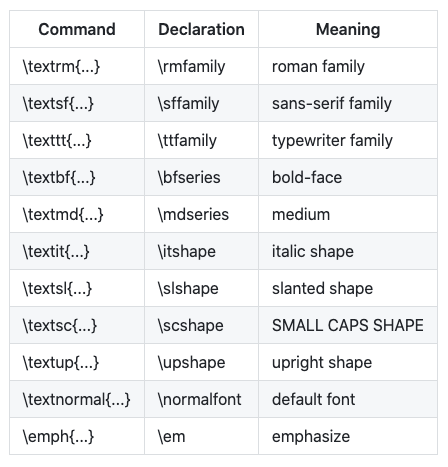
\includegraphics[scale=0.5]{image/commands.png}

{\sffamily
	Text is sans-serif. Text can be {\em emphasized}.
}

{\fontfamily{qcs}\selectfont
	This text uses a different font typeface
}

Normal text, {\sffamily sans serif text {\bfseries and bold}}.

\section{Indent}

Paragraphs will be automatically indented.

\begin{verbatim}
Use \setlength\parindent{0pt} for noindent throughout the document.

Use \noindent for part of document.

\end{verbatim}

\section{Columns}
\begin{verbatim}
Use \documentclass{proc} for two columns format.
\end{verbatim}

\subsection{Commenting}
\begin{verbatim}
Use % for comments.

\end{verbatim}

\subsection{Other notes}
\begin{verbatim}
'\,' 1\,cm
\end{verbatim}

\end{document}